\section{Fallbeispiel: Der Zahllauf}\label{chap:paymentrun}

Im Bereich der Geschäftsanwendungen gibt es eine Reihe hochkomplexer Prozesse, die in der IT abgebildet werden.
Einer davon ist der sogenannte Zahllauf, bei dem sich der Anwender eine Liste von offenen Zahlungen erst vorschlagen lässt und anschließend die Bearbeitung durch das System veranlasst.
Dabei spielen die Abhängigkeiten von Zahlungen, Lieferanten und Rabattverträgen eine wichtige Rolle, da sie im Idealfall in einer günstigen Konstellation für das Unternehmen resultieren und dadurch Einsparungen bei den Ausgaben ermöglichen.

Aus diesem Grund hat die Implementierung des dazugehörigen Algorithmus viele Einflussfaktoren. 
Zusätzlich erschweren große Relationen stark abgekürzten Feldern und Werten, die als Eingabe, Zwischenspeicher und Ausgabe dienen, das Erstellen einer daten- und performancebewussten Umsetzung besonders für domänenfremde Entwickler.
Umso wichtiger ist es bereits frühzeitig in der Entwicklung relevante Testdaten zu nutzen, die auch Randfälle der Implementierung abdecken und Engpässe aufzeigen.
Dabei unterstützt die im Rahmen des Bachelorprojektes erstellte Web-IDE durch die in dieser Arbeit vorgestellten Ansätze zur Generierung von Testdatenvorschlägen.

In diesem Kapitel wird exemplarisch die Implementierung des Zahllauf-Algorithmus mithilfe der Web-IDE vorgestellt.
Dabei steht die von Nutzereingaben geprägte Verarbeitung der Suchanfrage im Fokus.
Auf dieser Grundlage wird anschließend eine Evaluierung der vorgestellten Ansätze zum Vorgeschlagen von Testwerten durchgeführt.

\subsection{Implementierung des Algorithmus in der Web-IDE}

\begin{figure}[ht]
	\centering
  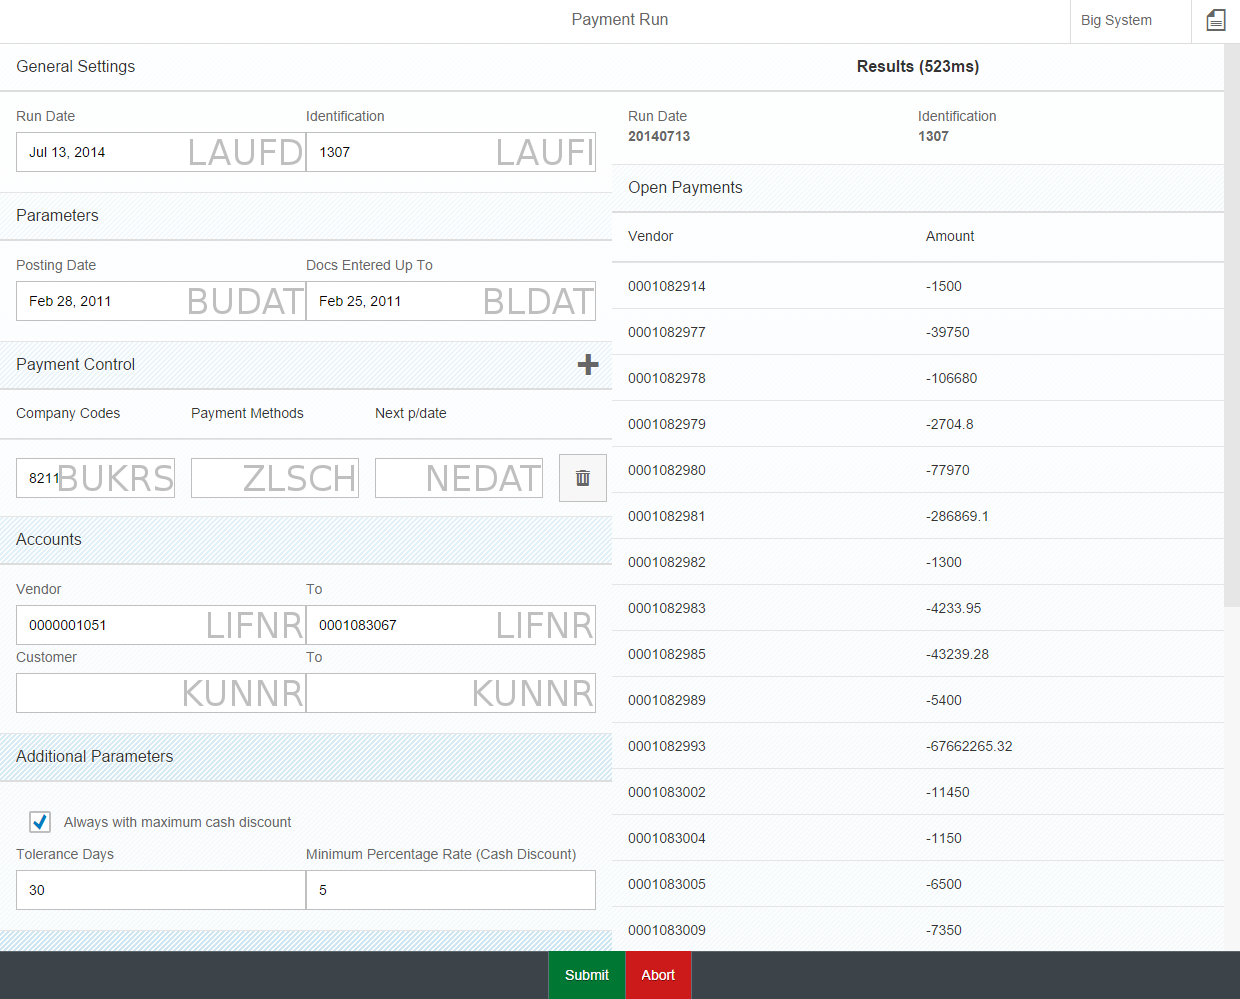
\includegraphics[width=1\textwidth]{figures/paymentrun.png}
	\caption{Eingabemaske des Zahllaufs}
	\label{fig:paymentrun}
\end{figure}

\nomenclature{UI}{User Interface}
Die in Abbildung \ref{fig:paymentrun} dargestellte Filtereingabemaske des Zahllaufs besteht zum einen aus allgemeinen Parametern für die Suche und zum anderen aus Eingabefeldern für Suchkriterien einzelner Rechnungen.
Für die Implementierung des Frontends wurde das UI-Framework OpenUI5\footnote{\url{http://sap.github.io/openui5/}} von SAP genutzt, der Fokus dieses Kapitels liegt indessen auf der Backendimplementierung mittels der SAP XS-Engine\footnote{\url{http://help.sap.com/hana/SAP_HANA_XS_JavaScript_Reference_en/index.html}}.

Der Algorithmus des Zahllaufs besteht aus 5 Schritten:
   \begin{enumerate}
      \item Parsen der JSON-Anfrage vom Frontend
			\item Selektion von Belegpositionen und Speicherung in der REGUP-Relation
			\item Berechnung von Zahldatum und Skonto
			\item Speicherung der Beleginformationen in der REGUH-Relation
			\item Senden einer JSON-Antwort
   \end{enumerate}

Die Eingaben des Nutzers in der Filtermaske (aus dem 1. Schritt, siehe Code-Beispiel \ref{lst:jsoninput} im Anhang) wirken sich insbesondere auf die Selektion der Belegpositionen aus.
Dem allgemeinen Teil des dazugehörigen SQL-Statements (siehe Code-Beispiel \ref{lst:regupgeneral} im Anhang) werden durch die Eingaben weitere Filterkriterien hinzugefügt, die nachfolgend näher untersucht werden.

Das Code-Beispiel \ref{lst:laufi} zeigt exemplarisch, wie die Projektion des Ausführungsdatums (zu sehen in Abbildung \ref{fig:paymentrun} unter ``General Settings'') dem SQL-Statement ergänzt werden.
Für das Identifikationsmerkmal (\texttt{LAUFI}) gilt dies analog.

\begin{lstlisting}[caption={Ergänzung der Projektion im SQL-Statement um das Ausführungsdatum für den Zahllauf}, label={lst:laufi}, language=JavaScriptSQL]
	if(oRunDate){
			insertRegup += SQL SELECT @oRunDate as LAUFD;
	} else {
			insertRegup += SQL SELECT '' as LAUFD;
	}
\end{lstlisting}

Anschließend werden dem SQL-Statement optional die Filter für Buchungs- und Erfassungsdatum (unter ``Parameters'' in Abbildung \ref{fig:paymentrun}) hinzugefügt (Code-Beispiel \ref{lst:budat}).

\begin{lstlisting}[caption={Einfügung von zusätzlichen Filtern}, label={lst:budat}, language=JavaScriptSQL]
	if(oPostingDate){
			insertRegup += SQL WHERE AND BSEG.BUDAT = @oPostingDate;
	}
	if(oDocsEnteredDate){
			insertRegup += SQL WHERE AND BSEG.BLDAT <= @oDocsEnteredDate;
	}
\end{lstlisting}

Für die Eingabe von einer bzw. mehreren Kundennummern (in Abbildung \ref{fig:paymentrun} unter ``Accounts'' ) wird das bereits bekannte Code-Beispiel \ref{lst:newsql} aus Kapitel \ref{sec:sqlandsourcecode} genutzt und kann in leicht abgewandelter Form auch für Lieferantennummern verwendet werden.

\begin{lstlisting}[caption={Unterscheidung zwischen Einzel- und Bereichsfilter}, label={lst:vendor}, language=JavaScriptSQL]
	if(oTextInputVendor && !oTextInputVendorTo ){
			insertRegup += SQL WHERE AND BSEG.LIFNR = @oTextInputVendor;
	}
	if(oTextInputVendor && oTextInputVendorTo ){
			insertRegup += SQL WHERE AND BSEG.LIFNR BETWEEN @oTextInputVendor
				AND @oTextInputVendorTo;
	}
\end{lstlisting}

Das komplexeste Konstrukt der Eingabemaske ist die Tabelle für Kriterien zur Suche anhand von Buchungskreisen, Zahlmethoden und dem nächsten Ausführungsdatums des Zahllaufs.
Die einzelnen Zellen einer Reihe bilden eine Konjunktion, wobei die Reihen miteinander disjunkt sind.
Die Komplexität entsteht durch die vielen Möglichkeiten der Eingabe.
So können Buchungskreise z.B. kommasepariert, mittels Klammern als Bereich oder beides kombiniert angegeben werden.
Die Zahlmethoden werden mit Großbuchstaben abgekürzt und aneinander gereiht um mehrere Methoden zuzulassen.

Die Verarbeitung der Nutzereingaben aus der Tabelle erfolgt zeilenweise.
Für jede Zeile wird ein leeres SQL-Statement erstellt.
Dieses wird im ersten Schritt mit den, mittels der Funktion \texttt{parseCompanyCodes()} ermittelten, Buchungskreisen gefüllt.
Sollten Zahlmethoden und ein nächstes Ausführungsdatum angegeben sein, werden diese dem SQL-Statement ergänzt.
Anschließend wird es einem allgemeinen, anfangs leeren SQL-Statement hinzugefügt.
Sobald alle Zeilen der Tabelle abgearbeitet sind, wird der zusammengestellte Filter dem SQL-Statement \texttt{insertRegup} angefügt.
Der Algorithmus zur Verarbeitung dieser Eingaben befindet sich im Anhang (Code-Beispiel \ref{lst:paymentcontrol}).

Die Berechnung vom Zahldatum und Skontobetrag erfolgt mithilfe einer SQLScript-Funktion im selben Schritt mit der Ermittlung und Speicherung der Beleginformationen in der REGUH-Relation.
Im letzten Schritt dienen der Ergebnisse in der REGUH-Relation für die JSON-Antwort an den Anwender.
Sie enthält eine Liste mit Gesamtbetrag, Lieferantennummer, Ausführungsdatum Identifikationsmerkmal für jede erfasste Rechnung der REGUH-Relation.

Die vielen optionalen Eingaben durch den Anwender bestimmen das Aussehen, die Komplexität und die Laufzeit des untersuchten SQL-Statements.
In diesen Fällen ist es für Entwickler deshalb wichtig relevante Testwerte zu haben, um früh in der Entwicklung Performance-Analysen zu ermöglichen.
Für das vorgestellte SQL-Statement werden dazu im folgenden Kapitel die Ansätze dieser Arbeit zur Vorschlagsgenerierung evaluiert.

\subsection{Evaluierung der vorgestellten Ansätze am Fallbeispiel}
% Die im Rahmen dieser Bachelorarbeit vorgestellten Ansätze zur Vorschlagsgenerierung von Testwerten werden in diesem Kapitel auf Basis des Fallbeispiels evaluiert.
Zur Evaluation der vorgestellten Ansätze wurde ein vergleichendes Experiment auf Basis des Fallbeispiels durchgeführt.
Dazu wurde das Verhältnis der durch die Algorithmen vorgeschlagenen Eingabetupel mit der Betrachtung aller Wertkombinationen (Brute-Force) untersucht.

Als Grundlage dienten folgende mögliche Nutzereingaben zur Filterung der Ergebnisse des Zahllaufprogramms:

   \begin{itemize}
      \item Buchungsdatum (\texttt{BUDAT})
      \item Belegdatum (\texttt{BLDAT})
			\item Lieferantennummer (\texttt{LIFNR})
			\item Zahlmethode (\texttt{ZLSCH})
			\item Buchungskreis (\texttt{BUKRS})
   \end{itemize}
	
Die ermittelten Vorschläge nach dem im Kapitel \ref{chap:datacharacteristics} spezifizierten Verfahren sind in den Tabellen \ref{tab:paymentruntable1}, \ref{tab:paymentruntable2} und \ref{tab:paymentruntable3} dargestellt (siehe Anhang).
Naheliegend ist die Auswahl der häufigsten Werte der jeweiligen Spalten für eine Analyse der Datenbankanfrage, welche jedoch eine leere Ergebnismenge liefert.
Deshalb wird in der adaptiven Erweiterung des Ansatzes (siehe Kapitel \ref{chap:adaptive}) die Bildung initialer Kombinationen der ermittelten Testwerte als Testdatensets vorgenommmen.
Tabelle \ref{tab:tupel} zeigt die zwei in diesem Schritt gefundenen Tupel, die beim Ausführen der Datenbankanfrage mindestens eine Ergebniszeile zurückgeben, mitsamt ihren Ausführungszeiten.
\begin{table}[h]
	\centering
	\scalebox{.9}{
	\begin{tabular}{ |c|c|c|c|c|c|c| }
		\hline
		\texttt{BUDAT} & \texttt{BLDAT} & \texttt{LIFNR} & \texttt{ZLSCH} & \texttt{BUKRS} & Ergebnisse & Zeit (ms) \\
		\hline
		'20110228' & '20101208' & '0001082993' & ' ' & '8211' & 231 & 49,917 \\
		'20110228' & '20101204' & '0001082993' & ' ' & '8211' & 117 & 49,280 \\
		\hline
	\end{tabular}
	}
	\caption{Gefundene Tupel für Testdatensets}
	\label{tab:tupel}
\end{table}

Vergleicht man die ermittelten Testdatensets mit den initial vorgeschlagenen häufigsten Werten der einzelnen Spalten, fällt auf, dass die Werte des Buchungsdatums, der Lieferantennummer, der Zahlmethode und des Buchungskreises konstant bleiben und nur das Belegdatum in seinem Wert variiert.
Des Weiteren ist zu beobachten, dass alle Werte aus den ermittelten Listen der häufigsten Werte stammen.
Dies kann mit der Verteilung der Daten begründet werden, dargestellt in den Abbildungen \ref{fig:budatverteilung} bis \ref{fig:zlschverteilung} (siehe Anhang).
Die Grafiken zeigen das Verhältnis von der Anzahl distinkter Werten innerhalb einer Spalte zu der Anzahl der Ausprägungen in den Einträgen der Relation.
Beispielsweise haben 630 distinkte Werte in der Spalte \texttt{BUDAT} nur jeweils einen Eintrag, wohingegen ein einziger Wert 760 Repräsentationen in der Relation hat.

Dies zeigt sich auch in den Abbildungen \ref{fig:budatverteilung} (\texttt{BUDAT}), \ref{fig:bldatverteilung} (\texttt{BLDAT}) und \ref{fig:lifnrverteilung} (\texttt{LIFNR}).
Es wird deutlich, dass die Mehrheit der gefunden distinkten Werte in den Spalten meist nur in einem Eintrag der Relation genutzt werden.
Dem gegenüber stehen wenige Ausnahmen, die eine hohe Anzahl von Repräsenationen innerhalb der Relation umfassen.
Dies zeichnet sich auch in den ermittelten, vorgeschlagenen Werten um den Median ab (Tabelle \ref{tab:paymentruntable3}), bei der die Werte für die Spalten \texttt{BUDAT}, \texttt{BLDAT} und \texttt{LIFNR} auch dort nur einen Eintrag vorweisen.

Ebenso zeigen die Verteilung der Daten in den Spalten \texttt{BUKRS} und \texttt{ZLSCH} (Abbildung \ref{fig:bukrsverteilung} und \ref{fig:zlschverteilung}) eine deutlich Spaltung.
So ist zu erkennen, dass jeweils ein Wert im Großteil der Einträge in der Relation genutzt wird und somit die anderen distinkten Werte nur wenige Ausprägungen haben.
Aufgrund der wenigen distinkten Werte ergibt dies eine Gerade in der Darstellung.

Zum Vergleich würde die Betrachtung aller Wertkombinationen das Erzeugen einer Permutation über alle Listen der distinkten Werte der fünf betrachteten Spalten erfordern.
Aufgrund der Größe der einzelnen Listen (\texttt{BUDAT} 903, \texttt{BLDAT} 933, \texttt{LIFNR} 247, \texttt{ZLSCH} 6, \texttt{BUKRS} 9) ergäbe sich in der Gesamtsumme ein Liste mit über 11,2 Milliarden Einträgen.
Des Weiteren hat nur ein Bruchteil dieser Kombinationen mindestens einen Repräsentanten in der Datenbank.
In der Annahme, dass die Berechnung der Analyse pro Listeneintrag 10ms braucht, entspräche dies über 3 Jahre Berechnungen.

Aus diesem Grund fokussiert sich das Experiment auf den Vergleich der Ergebnisse folgender Ansätze:

   \begin{enumerate}
      \item Adaptiver Algorithmus mit fester Obergrenze (50)
      \item Adaptiver Algorithmus ohne feste Obergrenze
			\item Permutation der ermittelten häufigste, seltensten und mittleren Werte der Spalten
   \end{enumerate}

Dazu wird ermittelt, welcher der Ansätze die meisten der 5 Tupel mit den größten Ergebnismengen ermittelt (zu sehen in Tabelle \ref{tab:tupel2}).
Dies wird zusätzlich in Beziehung zu der Anzahl der betrachteten Tupel und die Laufzeit der Ermittlung betrachtet.

\begin{table}[h]
	\centering
	\scalebox{.85}{
	\begin{tabular}{ |c|c|c|c|c|c|c|c| }
		\hline
		Tupel & \texttt{BUDAT} & \texttt{BLDAT} & \texttt{LIFNR} & \texttt{ZLSCH} & \texttt{BUKRS} & Ergebnisse & Zeit (ms)\\
		\hline
        1 & '20110228' & '20101227' & '0001082993' & ' ' & '8211' & 234 & 52,317 \\
        2 & '20110228' & '20101220' & '0001082993' & ' ' & '8211' & 233 & 51,689 \\
        3 & '20110228' & '20101213' & '0001082993' & ' ' & '8211' & 232 & 50,240 \\
        4 & '20110228' & '20101208' & '0001082993' & ' ' & '8211' & 231 & 49,917 \\
        5 & '20110228' & '20101204' & '0001082993' & ' ' & '8211' & 117 & 49,280 \\
		\hline
	\end{tabular}
	}
	\caption{Eingabetupel für mit den meisten Ergebnissen}
	\label{tab:tupel2}
\end{table}

Die Ergebnisse (Tabelle \ref{tab:tupel3}) zeigen, dass die Einschränkung durch die Obergrenze den Umfang der gefunden Tupel reduziert.
Die Betrachtung der Permutation ergibt zwar einen Tupel mehr, benötigt aber über eine Halbe Minute, da mehr als 30.000 Tupel getestet werden.

\begin{table}[h]
	\centering
	\scalebox{.75}{
	\begin{tabular}{ |c|c|c|c|c|c|c|c|c| }
		\cline{2-8}
		\multicolumn{1}{c|}{} & Tupel 1 & Tupel 2 & Tupel 3 & Tupel 4 & Tupel 5 & Getestete Tupel & Laufzeit (sek)\\
		\hline
        mit Obergrenze &  &  &  & X & X & 50 & 0,058 \\
        ohne Obergrenze & X & X & X & X & X & 1.860 & 2,239 \\
        Permutation & X &  &  & X & X & 30.618 & 34,352 \\
		\hline
	\end{tabular}
	}
	\caption{Vergleich der Ansätze}
	\label{tab:tupel3}
\end{table}

Der Grund für vollständige Abdeckung der Tupel der Variante ohne Obergrenze liegt in der Ermittlung der zu testenden Tupel.
Die 1.860 bestimmten Tupel entsprechen allen distinkten Konstellationen der Werte der betrachteten Spalten.
Davon haben insgesamt nur 301 mindestens eine Ergebniszeile beim Ausführen des Programms, was einer Abdeckung des kompletten Eingaberaums entspricht.
Die Festlegung einer Obergrenze entspricht also einer Einschränkung auf einen Subraum.
Die Verteilung der 301 Tupel (siehe Abbildung \ref{fig:tupelverteilung}) macht deutlich, dass der Großteil der Eingabekonstellationen nur eine Ergebniszeile aus der Datenbank zurückgeben (187 Tupel) und nur wenige Tupel eine größere Ergebnismenge abrufen (5 Tupel mit über 150 Ergebnissen, erfasst in Tabelle \ref{tab:tupel2}).
Dies spiegelt die zuvor betrachtete Verteilung der Daten innerhalb der einzelnen Spalten wieder.

Aufgrund dessen ist es in Erwägung zu ziehen dem Entwickler die Möglichkeit der Festlegung einer Obergrenze zu geben.
Dies bedarf weiteren Untersuchungen in Hinblick auf die Beziehung zwischen der Anzahl der betrachteten Spalten, dem Umfang an distinkten Werten und der Laufzeit der Berechnungen.

\begin{figure}[ht]
\centering
	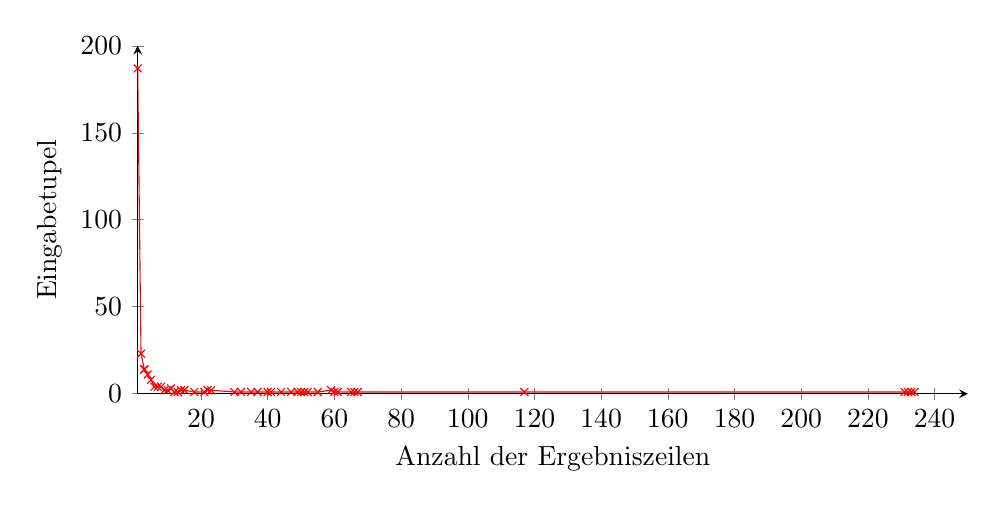
\begin{tikzpicture}
		\begin{axis}[
				axis lines=left,
				width  = 1*\textwidth,
				height  = 6cm,
				%symbolic x coords={1,2,3,4,5,6,7,8,9,10,11,12,13,14,15,15,18,21,22,23,30,32,35,37,40,41,44,47,49,50,51,52,55,59,60,61,65,66,67,117,231,232,233,234},
				%xtick=data,
				%enlarge x limits=0.05,
				%bar width=5pt,
				%ybar,
				ylabel={Eingabetupel},
				xlabel={Anzahl der Ergebniszeilen},
				ymin=0.0,
				ymax=200.0,
				xmax=250.0,
				]
				%\addplot[ybar,fill=light-gray] coordinates {
				\addplot[color=red,mark=x] coordinates {
						(1,187)
						(2,23)
						(3,14)
						(3,14)
						(4,11)
						(5,8)
						(6,4)
						(7,4)
						(8,4)
						(9,2)
						(10,2)
						(11,3)
						(12,1)
						(13,1)
						(14,2)
						(15,2)
						(15,2)
						(18,1)
						(21,1)
						(22,2)
						(23,2)
						(30,1)
						(32,1)
						(35,1)
						(37,1)
						(40,1)
						(41,1)
						(44,1)
						(47,1)
						(49,1)
						(50,1)
						(51,1)
						(52,1)
						(55,1)
						(59,2)
						(60,1)
						(61,1)
						(65,1)
						(66,1)
						(67,1)
						(117,1)
						(231,1)
						(232,1)
						(233,1)
						(234,1)
				};
		\end{axis}
	\end{tikzpicture}
	\caption{Verteilung der Ergebnisszeilen in Relation zu den Eingabetupeln}
	\label{fig:tupelverteilung}
\end{figure}

Die derzeitige adaptive Lösung ermöglicht es auf Grundlage der mit Obergrenze ermittelten initialen Testdatensets durch exploratives Erweiterung durch den Entwickler den ermittelten Datensatz zu ergänzen.

%\begin{table}[h]
	%\centering
	%\scalebox{.9}{
	%\begin{tabular}{ |c|c|c|c|c|c|c| }
		%\hline
		%\texttt{BUDAT} & \texttt{BLDAT} & \texttt{LIFNR} & \texttt{ZLSCH} & \texttt{BUKRS} & Ergebnisse & Zeit (ms)\\
		%\hline
		%\textbf{'20110228'} & \textbf{'20110216'} & \textbf{'0001082993'} & \textbf{' '} & \textbf{'8211'} & \textbf{234} & \textbf{52,317} \\
		%'20110228' & '20101220' & '0001082993' & ' ' & '8211' & 233 & 51,689 \\
		%'20110228' & '20110216' & '0001082993' & ' ' & '8211' & 232 & 50,240 \\
		%\textbf{'20110228'} & \textbf{'20101213'} & \textbf{'0001082993'} & \textbf{' '} & \textbf{'8211'} & \textbf{231} & \textbf{49,917} \\
		%\textbf{'20110228'} & \textbf{'20101204'} & \textbf{'0001082993'} & \textbf{' '} & \textbf{'8211'} & \textbf{117} & \textbf{49,280} \\
		%\hline
	%\end{tabular}
	%}
	%\caption{Gefundene Tupel für Testdatensets}
	%\label{tab:tupel2}
%\end{table}

%Die Messergebnisse zeigen, dass 3 der 5 Kombinationen von Eingabewerten mit den höchsten Ergebnismengen und Laufzeiten durch die vorgestellten Ansätze vorgeschlagen wurden (in Tabelle \ref{tab:tupel2} dick hervorgehoben).
%Im Vergleich mussten dazu jediglich 
%Zusätzlich kann die adaptive Variantedurch exploratives Probieren weitere Testwerte durch den Entwickler dem ermittelten Datensatz ergänzen.
